\documentclass{standalone}
\usepackage{tikz}
\usetikzlibrary{patterns, positioning}
\usepackage[sfdefault]{ClearSans} %% option 'sfdefault' activates Clear Sans as the default text font
\usepackage[T1]{fontenc}

\begin{document}
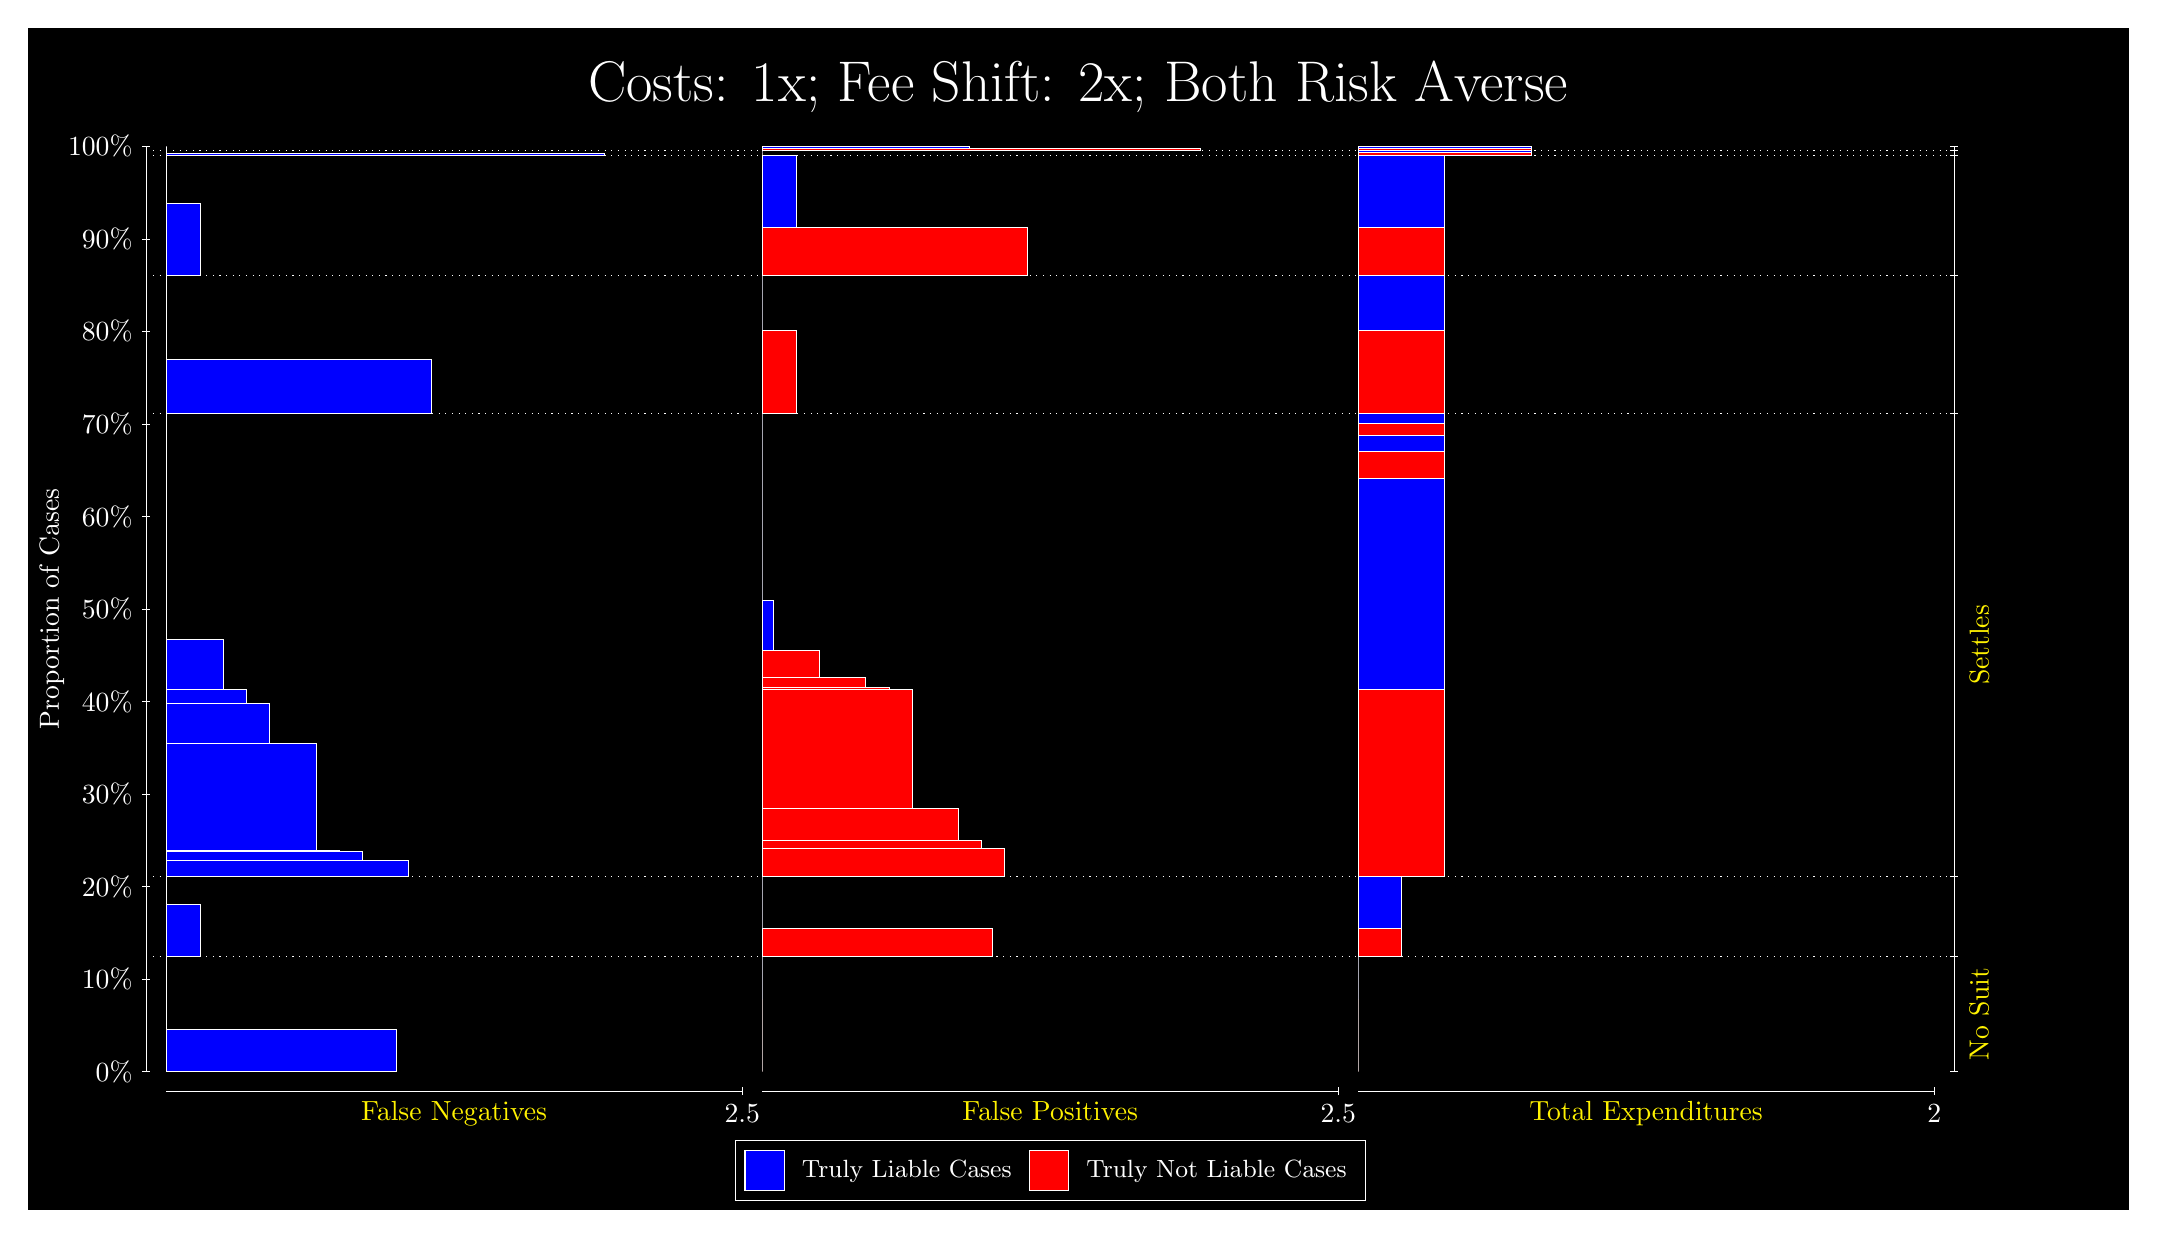
\begin{tikzpicture}
\draw[fill=black] (0,0) rectangle (26.667,15);
\draw[text=white] (0,13.5) rectangle (26.667,15) node[midway] {\huge Costs: 1x; Fee Shift: 2x; Both Risk Averse};
\draw[white, very thin] (1.5,1.75) -- (1.5,13.5);
\node[rotate=90, text=white, anchor=center] at (0.3, 7.625) {Proportion of Cases};
\draw[white, very thin] (1.45,1.75) -- (1.55,1.75);
\node[text=white, anchor=east] at (1.45, 1.75) {0\%};
\draw[white, very thin] (1.45,2.925) -- (1.55,2.925);
\node[text=white, anchor=east] at (1.45, 2.925) {10\%};
\draw[white, very thin] (1.45,4.1) -- (1.55,4.1);
\node[text=white, anchor=east] at (1.45, 4.1) {20\%};
\draw[white, very thin] (1.45,5.275) -- (1.55,5.275);
\node[text=white, anchor=east] at (1.45, 5.275) {30\%};
\draw[white, very thin] (1.45,6.45) -- (1.55,6.45);
\node[text=white, anchor=east] at (1.45, 6.45) {40\%};
\draw[white, very thin] (1.45,7.625) -- (1.55,7.625);
\node[text=white, anchor=east] at (1.45, 7.625) {50\%};
\draw[white, very thin] (1.45,8.8) -- (1.55,8.8);
\node[text=white, anchor=east] at (1.45, 8.8) {60\%};
\draw[white, very thin] (1.45,9.975) -- (1.55,9.975);
\node[text=white, anchor=east] at (1.45, 9.975) {70\%};
\draw[white, very thin] (1.45,11.15) -- (1.55,11.15);
\node[text=white, anchor=east] at (1.45, 11.15) {80\%};
\draw[white, very thin] (1.45,12.325) -- (1.55,12.325);
\node[text=white, anchor=east] at (1.45, 12.325) {90\%};
\draw[white, very thin] (1.45,13.5) -- (1.55,13.5);
\node[text=white, anchor=east] at (1.45, 13.5) {100\%};

\draw[white, very thin] (24.457,1.75) -- (24.457,13.5);
\draw[white, very thin] (24.407,1.75) -- (24.507,1.75);
\node[anchor=west] at (24.407, 1.75) {};
\draw[white, very thin] (24.407,3.2091) -- (24.507,3.2091);
\node[anchor=west] at (24.407, 3.2091) {};
\draw[white, very thin] (24.407,4.2269) -- (24.507,4.2269);
\node[anchor=west] at (24.407, 4.2269) {};
\draw[white, very thin] (24.407,10.11) -- (24.507,10.11);
\node[anchor=west] at (24.407, 10.11) {};
\draw[white, very thin] (24.407,11.856) -- (24.507,11.856);
\node[anchor=west] at (24.407, 11.856) {};
\draw[white, very thin] (24.407,13.388) -- (24.507,13.388);
\node[anchor=west] at (24.407, 13.388) {};
\draw[white, very thin] (24.407,13.444) -- (24.507,13.444);
\node[anchor=west] at (24.407, 13.444) {};
\draw[white, very thin] (24.407,13.5) -- (24.507,13.5);
\node[anchor=west] at (24.407, 13.5) {};

\draw[white, very thin, fill=blue] (1.75,1.75) rectangle (4.6775,2.2894);
\draw[white, very thin, fill=red] (1.75,2.2894) rectangle (1.75,3.2091);
\draw[white, very thin, fill=blue] (1.75,3.2091) rectangle (2.1891,3.8682);
\draw[white, very thin, fill=red] (1.75,3.8682) rectangle (1.75,4.2269);
\draw[white, very thin, fill=blue] (1.75,4.2269) rectangle (4.8239,4.4325);
\draw[white, very thin, fill=blue] (1.75,4.4325) rectangle (4.2384,4.5479);
\draw[white, very thin, fill=blue] (1.75,4.5479) rectangle (3.9457,4.5635);
\draw[white, very thin, fill=blue] (1.75,4.5635) rectangle (3.6529,5.9229);
\draw[white, very thin, fill=blue] (1.75,5.9229) rectangle (3.0674,6.4325);
\draw[white, very thin, fill=blue] (1.75,6.4325) rectangle (2.7746,6.6017);
\draw[white, very thin, fill=blue] (1.75,6.6017) rectangle (2.4819,7.2388);
\draw[white, very thin, fill=red] (1.75,7.2388) rectangle (1.75,10.11);
\draw[white, very thin, fill=blue] (1.75,10.11) rectangle (5.1167,10.8);
\draw[white, very thin, fill=red] (1.75,10.8) rectangle (1.75,11.856);
\draw[white, very thin, fill=blue] (1.75,11.856) rectangle (2.1891,12.774);
\draw[white, very thin, fill=red] (1.75,12.774) rectangle (1.75,13.388);
\draw[white, very thin, fill=blue] (1.75,13.388) rectangle (7.3123,13.413);
\draw[white, very thin, fill=red] (1.75,13.413) rectangle (1.75,13.444);
\draw[white, very thin, fill=red] (1.75,13.444) rectangle (1.75,13.469);
\draw[white, very thin, fill=blue] (1.75,13.469) rectangle (1.75,13.5);
\draw[white, very thin, fill=red] (9.3189,1.75) rectangle (9.3189,2.6697);
\draw[white, very thin, fill=blue] (9.3189,2.6697) rectangle (9.3189,3.2091);
\draw[white, very thin, fill=red] (9.3189,3.2091) rectangle (12.246,3.5678);
\draw[white, very thin, fill=blue] (9.3189,3.5678) rectangle (9.3189,4.2269);
\draw[white, very thin, fill=red] (9.3189,4.2269) rectangle (12.393,4.5879);
\draw[white, very thin, fill=red] (9.3189,4.5879) rectangle (12.1,4.6841);
\draw[white, very thin, fill=red] (9.3189,4.6841) rectangle (11.807,5.0975);
\draw[white, very thin, fill=red] (9.3189,5.0975) rectangle (11.222,6.6097);
\draw[white, very thin, fill=red] (9.3189,6.6097) rectangle (10.929,6.6264);
\draw[white, very thin, fill=red] (9.3189,6.6264) rectangle (10.636,6.7563);
\draw[white, very thin, fill=red] (9.3189,6.7563) rectangle (10.051,7.0977);
\draw[white, very thin, fill=blue] (9.3189,7.0977) rectangle (9.4652,7.7348);
\draw[white, very thin, fill=blue] (9.3189,7.7348) rectangle (9.3189,10.11);
\draw[white, very thin, fill=red] (9.3189,10.11) rectangle (9.758,11.165);
\draw[white, very thin, fill=blue] (9.3189,11.165) rectangle (9.3189,11.856);
\draw[white, very thin, fill=red] (9.3189,11.856) rectangle (12.686,12.47);
\draw[white, very thin, fill=blue] (9.3189,12.47) rectangle (9.758,13.388);
\draw[white, very thin, fill=red] (9.3189,13.388) rectangle (9.3189,13.419);
\draw[white, very thin, fill=blue] (9.3189,13.419) rectangle (9.3189,13.444);
\draw[white, very thin, fill=red] (9.3189,13.444) rectangle (14.881,13.469);
\draw[white, very thin, fill=blue] (9.3189,13.469) rectangle (11.954,13.5);
\draw[white, very thin, fill=red] (16.888,1.75) rectangle (16.888,2.6697);
\draw[white, very thin, fill=blue] (16.888,2.6697) rectangle (16.888,3.2091);
\draw[white, very thin, fill=red] (16.888,3.2091) rectangle (17.437,3.5678);
\draw[white, very thin, fill=blue] (16.888,3.5678) rectangle (17.437,4.2269);
\draw[white, very thin, fill=red] (16.888,4.2269) rectangle (17.986,6.6097);
\draw[white, very thin, fill=blue] (16.888,6.6097) rectangle (17.986,9.2849);
\draw[white, very thin, fill=red] (16.888,9.2849) rectangle (17.986,9.6264);
\draw[white, very thin, fill=blue] (16.888,9.6264) rectangle (17.986,9.832);
\draw[white, very thin, fill=red] (16.888,9.832) rectangle (17.986,9.9786);
\draw[white, very thin, fill=blue] (16.888,9.9786) rectangle (17.986,10.11);
\draw[white, very thin, fill=red] (16.888,10.11) rectangle (17.986,11.165);
\draw[white, very thin, fill=blue] (16.888,11.165) rectangle (17.986,11.856);
\draw[white, very thin, fill=red] (16.888,11.856) rectangle (17.986,12.47);
\draw[white, very thin, fill=blue] (16.888,12.47) rectangle (17.986,13.388);
\draw[white, very thin, fill=red] (16.888,13.388) rectangle (19.083,13.419);
\draw[white, very thin, fill=blue] (16.888,13.419) rectangle (19.083,13.444);
\draw[white, very thin, fill=red] (16.888,13.444) rectangle (19.083,13.469);
\draw[white, very thin, fill=blue] (16.888,13.469) rectangle (19.083,13.5);
\draw[white, dotted] (1.5,3.2091) -- (24.457,3.2091);
\draw[white, dotted] (1.5,4.2269) -- (24.457,4.2269);
\draw[white, dotted] (1.5,10.11) -- (24.457,10.11);
\draw[white, dotted] (1.5,11.856) -- (24.457,11.856);
\draw[white, dotted] (1.5,13.388) -- (24.457,13.388);
\draw[white, dotted] (1.5,13.444) -- (24.457,13.444);
\draw[white, very thin] (1.75,1.5) -- (9.0689,1.5);
\node[text=yellow, anchor=north] at (5.4094, 1.5) {False Negatives};
\draw[white, very thin] (9.0689,1.45) -- (9.0689,1.55);
\node[text=white, anchor=north] at (9.0689, 1.45) {2.5};

\draw[white, very thin] (9.3189,1.5) -- (16.638,1.5);
\node[text=yellow, anchor=north] at (12.978, 1.5) {False Positives};
\draw[white, very thin] (16.638,1.45) -- (16.638,1.55);
\node[text=white, anchor=north] at (16.638, 1.45) {2.5};

\draw[white, very thin] (16.888,1.5) -- (24.207,1.5);
\node[text=yellow, anchor=north] at (20.547, 1.5) {Total Expenditures};
\draw[white, very thin] (24.207,1.45) -- (24.207,1.55);
\node[text=white, anchor=north] at (24.207, 1.45) {2};

\node[text=yellow, centered, rotate=90] at (24.777, 2.4796) {No Suit};

\node[text=yellow, centered, rotate=90] at (24.777, 7.1682) {Settles};





\draw (12.978300999999998,1.5) node[draw=none] (baseCoordinate) {};
\begin{scope}[align=center]
        \matrix[scale=0.5, draw=white, below=0.5cm of baseCoordinate, nodes={draw}, column sep=0.1cm]{
            \node[rectangle, draw, minimum width=0.5cm, minimum height=0.5cm, fill=blue] {}; &
            \node[draw=none, font=\small, text=white] (B) {Truly Liable Cases}; &
            \node[rectangle, draw, minimum width=0.5cm, minimum height=0.5cm, fill=red] {}; &
            \node[draw=none, font=\small, text=white] (B) {Truly Not Liable Cases}; \\
            };
\end{scope}

\end{tikzpicture}
\end{document}